\documentclass[12pt,a4paper]{report}

\usepackage[left=2cm, right=2cm, top=4cm, bottom=2cm]{geometry}
\usepackage{enumitem}
\usepackage{fontspec}
\usepackage{tikz}
\usepackage{amsmath}

\begin{document}
	%Portada
	\begin{titlepage}
		\centering
		{\scshape\LARGE Universidad Nacional Autónoma de México \par}
		\vspace{1cm}
		{\scshape\Large Computación Distribuida\par}
		\vspace{1.5cm}
		{\huge\bfseries Tarea 7\par}
		\vspace{.5cm}
		{\Large\itshape Edgar Quiroz Castañeda \par}
		\vspace{.5cm}
		{\Large\itshape Jerónimo Almeida Rodríguez \par}
		\vfill
		 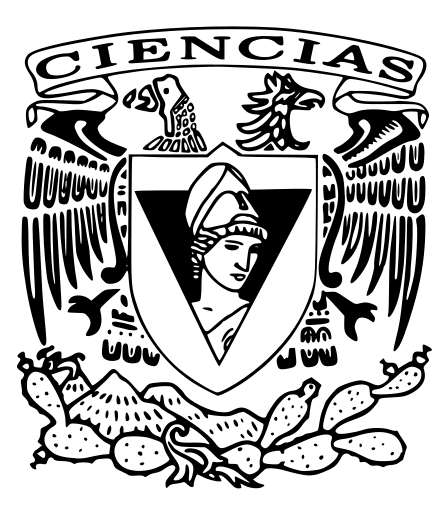
\includegraphics[width=0.5\textwidth]{escudo_f-ciencias.png}
		\vfill

		{\large Jueves 1 de noviembre del 2018 \par}
	\end{titlepage}

	\pagebreak
	\setlength{\voffset}{-0.75in}
	\setlength{\headsep}{5pt}

	%Ejercicios
	\begin{enumerate}
		%1
		\item {
			Considera la ejecución $\alpha$ de la Figura 1. Los retardos máximos
			para cada uno de los eventos son $B_{i, j}$, donde $i$ es el evento
			que envía y $j$ el que recibe.
			\begin{enumerate}
				%a
				\item {
					¿Cuánto vale el retardo máximo de $c$ a $e$ en términos de
					las $B$s? Es decir, dado $real(c)-real(e) \leq x$, ¿cuánto
					vale $x$?
				}

				%b
				item {
					Anotar los eventos con los relojes escalares y los relojes
					vectoriales.
				}

				%c
				\item {
					¿Cuáles son eventos concurrentes y cuáles no?
				}

				%d
				\item {
					Describe todos los cortes consistentes de $\alpha$.
				}
			\end{enumerate}
		}

		%2
		\item {
			Sea $G = (V, E)$ la gráfica dirigida de causalidad de una ejecución
			$\alpha$, $e, e' \in V$ y $L$ un reloj vectorial.\\
			Un evento causó a otro si existe un camino dirigido que inicia en
			el primer evento y acaba en el segundo.\\
			Demuestra que $e$ causó a $e'$ si y sólo si $L(e) < L(e')$.
		}

		%3
		\item {
			Lee los primeros 5 sueños del libro \textit{Einstein's Dream}.
			Redacta un pequeño resumen de cada uno de ellos.
		}

		%4
		\item {
			Sean $A$ y $B$ dos procesos cuyos relojes no están sincronizados,
			pero ambos tienen un $drift$ acotado. Un mensaje de $A$ a $B$
			tarda a lo más $D$, en tiempo real.\\
			Propón un algoritmo para que $B$ estime el tiempo de llegada de un
			mensaje de $A$, si este manda mensajes cada $T$ unidades de tiempo.
		}
	\end{enumerate}

\end{document}
